\documentclass{article}

\usepackage{fancyhdr} % Required for custom headers
\usepackage{lastpage} % Required to determine the last page for the footer
\usepackage{extramarks} % Required for headers and footers
\usepackage[usenames,dvipsnames]{color} % Required for custom colors
\usepackage{graphicx} % Required to insert images
\usepackage{listings} % Required for insertion of code
\usepackage{courier} % Required for the courier font
\usepackage{lipsum} % Used for inserting dummy 'Lorem ipsum' text into the template
\usepackage{amsmath}
\usepackage{amssymb}
\usepackage{mathtools, xparse}
\usepackage{booktabs}
\usepackage{bigstrut}
\usepackage{float}
\usepackage{hyperref}
\usepackage{color}
\usepackage{algorithm}
\usepackage{caption}
\usepackage{algpseudocode}
\usepackage{multirow}


\DeclarePairedDelimiter{\norm}{\lVert}{\rVert}
\DeclarePairedDelimiter\abs{\lvert}{\rvert}%

\hypersetup{
    colorlinks   = true,    % Colours links instead of ugly boxes
    urlcolor     = red,    % Colour for external hyperlinks
    linkcolor    = red,    % Colour of internal links
    citecolor    = red      % Colour of citations
}
% Margins
\topmargin=-0.45in
\evensidemargin=0in
\oddsidemargin=0in
\textwidth=6.5in
\textheight=9.0in
\headsep=0.25in

\linespread{1.1} % Line spacing

% Set up the header and footer
\pagestyle{fancy}
\lhead{\hmwkAuthorName} % Top left header
\chead{\hmwkClass\ : \hmwkID} % Top center head
\rhead{\firstxmark} % Top right header
\lfoot{\lastxmark} % Bottom left footer
\cfoot{} % Bottom center footer
\rfoot{Page\ \thepage\ of\ \protect\pageref*{LastPage}} % Bottom right footer
\renewcommand\headrulewidth{0.4pt} % Size of the header rule
\renewcommand\footrulewidth{0.4pt} % Size of the footer rule

\setlength\parindent{0pt} % Removes all indentation from paragraphs

%----------------------------------------------------------------------------------------
%	CODE INCLUSION CONFIGURATION
%----------------------------------------------------------------------------------------

\definecolor{MyDarkGreen}{rgb}{0.0,0.4,0.0} % This is the color used for comments
\lstloadlanguages{Perl} % Load Perl syntax for listings, for a list of other languages supported see: ftp://ftp.tex.ac.uk/tex-archive/macros/latex/contrib/listings/listings.pdf
\lstset{language=Perl, % Use Perl in this example
    frame=single, % Single frame around code
    basicstyle=\small\ttfamily, % Use small true type font
    keywordstyle=[1]\color{Blue}\bf, % Perl functions bold and blue
    keywordstyle=[2]\color{Purple}, % Perl function arguments purple
    keywordstyle=[3]\color{Blue}\underbar, % Custom functions underlined and blue
    identifierstyle=, % Nothing special about identifiers                                         
    commentstyle=\usefont{T1}{pcr}{m}{sl}\color{MyDarkGreen}\small, % Comments small dark green courier font
    stringstyle=\color{Purple}, % Strings are purple
    showstringspaces=false, % Don't put marks in string spaces
    tabsize=5, % 5 spaces per tab
    %
    % Put standard Perl functions not included in the default language here
    morekeywords={rand},
    %
    % Put Perl function parameters here
    morekeywords=[2]{on, off, interp},
    %
    % Put user defined functions here
    morekeywords=[3]{test},
    %
    morecomment=[l][\color{Blue}]{...}, % Line continuation (...) like blue comment
    numbers=left, % Line numbers on left
    firstnumber=1, % Line numbers start with line 1
    numberstyle=\tiny\color{Blue}, % Line numbers are blue and small
    stepnumber=5 % Line numbers go in steps of 5
}

% Creates a new command to include a perl script, the first parameter is the filename of the script (without .pl), the second parameter is the caption
\newcommand{\perlscript}[2]{
    \begin{itemize}
        \item[]\lstinputlisting[caption=#2,label=#1]{#1.py}
    \end{itemize}
}
\newcommand{\cppscript}[1]{
    \begin{itemize}
        \item[]\lstinputlisting[]{#1}
    \end{itemize}
}

%----------------------------------------------------------------------------------------
%	DOCUMENT STRUCTURE COMMANDS
%	Skip this unless you know what you're doing
%----------------------------------------------------------------------------------------

% Header and footer for when a page split occurs within a problem environment
\newcommand{\enterProblemHeader}[1]{
    \nobreak\extramarks{#1}{#1 continued on next page\ldots}\nobreak
    \nobreak\extramarks{#1 (continued)}{#1 continued on next page\ldots}\nobreak
}

% Header and footer for when a page split occurs between problem environments
\newcommand{\exitProblemHeader}[1]{
    \nobreak\extramarks{#1 (continued)}{#1 continued on next page\ldots}\nobreak
    \nobreak\extramarks{#1}{}\nobreak
}

%\setcounter{secnumdepth}{0} % Removes default section numbers
\newcounter{homeworkProblemCounter} % Creates a counter to keep track of the number of problems

\newcommand{\homeworkProblemName}{}
\newenvironment{homeworkProblem}[1][Problem \arabic{homeworkProblemCounter}]{ % Makes a new environment called homeworkProblem which takes 1 argument (custom name) but the default is "Problem #"
    \stepcounter{homeworkProblemCounter} % Increase counter for number of problems
    \renewcommand{\homeworkProblemName}{#1} % Assign \homeworkProblemName the name of the problem
    \section{\homeworkProblemName} % Make a section in the document with the custom problem count
    \enterProblemHeader{\homeworkProblemName} % Header and footer within the environment
    }{
    \exitProblemHeader{\homeworkProblemName} % Header and footer after the environment
}

\newcommand{\problemAnswer}[1]{ % Defines the problem answer command with the content as the only argument
\noindent\framebox[\columnwidth][c]{\begin{minipage}{0.98\columnwidth}#1\end{minipage}} % Makes the box around the problem answer and puts the content inside
}

\newcommand{\homeworkSectionName}{}
\newenvironment{homeworkSection}[1]{ % New environment for sections within homework problems, takes 1 argument - the name of the section
    \renewcommand{\homeworkSectionName}{#1} % Assign \homeworkSectionName to the name of the section from the environment argument
    \subsection{\homeworkSectionName} % Make a subsection with the custom name of the subsection
    \enterProblemHeader{\homeworkProblemName\ [\homeworkSectionName]} % Header and footer within the environment
    }{
    \enterProblemHeader{\homeworkProblemName} % Header and footer after the environment
}

%----------------------------------------------------------------------------------------
%	NAME AND CLASS SECTION
%----------------------------------------------------------------------------------------

\newcommand{\hmwkID}{homework 09} % Assignment title
\newcommand{\hmwkTitle}{Spline Interpolations}
\newcommand{\hmwkDueDate}{Tuesday,\ May\ 2,\ 2017} % Due date
\newcommand{\hmwkClass}{Numerical Analysis} % Course/class
\newcommand{\hmwkClassTime}{10:30am} % Class/lecture time
\newcommand{\hmwkClassInstructor}{Jones} % Teacher/lecturer
\newcommand{\hmwkAuthorName}{102061149 Fu-En Wang} % Your name

%----------------------------------------------------------------------------------------
%	TITLE PAGE
%----------------------------------------------------------------------------------------

\title{
    \vspace{2in}
    \textmd{\textbf{\hmwkClass}}\\
    \textmd{\textbf{\hmwkID: \hmwkTitle}} \\
    \normalsize\vspace{0.1in}\small{Due\ on\ \hmwkDueDate}\\
    \vspace{3in}
}

\author{\textbf{\hmwkAuthorName}}
\date{} % Insert date here if you want it to appear below your name

%----------------------------------------------------------------------------------------

\begin{document}
\maketitle
\newpage

\section{Introduction}
In previous homework, we have used Lagrange to get the interpolated values of f301.dat. However, when using Lagrange, we can find 
that the error around the two side of support points is quite large. As a result, to reduce the interpolated error, we will
introduce \textbf{Spline Interpolation} in this project.
\subsection{Spline Interpolation}
For a given support points set and their second derivative $M$, the interpolated value is
\begin{align}
    &y(x) = \alpha_i + \beta_i(x-x_{i-1}) + \gamma_i(x-x_{i-1})^2 + \delta_i(x-x_{i-1})^3 \\
    &\alpha_i = y_{i-1} \\
    &\beta_i = \frac{y_i - y_{i-1}}{h_i} - \frac{h_i}{6}(M_i + 2M_{i-1}) \\
    &\gamma_i = \frac{M_{i-1}}{2} \\
    &\delta_i = \frac{M_i - M_{i-1}}{6h_i}
\end{align}
\subsection{Moment}
For calculate moment, we will model the problem into a linear system.
\begin{align}
    &\begin{bmatrix}
        2 & \lambda_0 & 0 & 0 & ... & 0 \\
        \mu_1 & 2 & \lambda_1 & 0 & ... & 0  \\
        0 & \mu_2 & 2 & \lambda_2 & ... & 0 \\
        . &  & ... &\\
        . & & ... & & 2 & \lambda_{n-1}\\
        0 & & ... & & \mu_{n} & 2
    \end{bmatrix}
    \begin{bmatrix}
        M_0 \\
        M_1 \\
        M_2 \\
        ... \\
        M_{n-1} \\
        M_n
    \end{bmatrix}
    =
    \begin{bmatrix}
        d_0 \\
        d_1 \\
        d_2 \\
        ... \\
        d_{n-1} \\
        d_n
    \end{bmatrix} \\
    &\mu_i = \frac{h_i}{h_i + h_{i+1}} \\
    &\lambda_i = \frac{h_{i+1}}{h_i + h_{i+1}} \\
    &d_i = \frac{6}{h_i + h_{i+1}}(\frac{y_{i+1}-y_i}{h_{i+1}} - \frac{y_i-y_{i-1}}{h_i})
\end{align}
In this project, I use \textbf{zero boundary condition}
\begin{align*}
    &\lambda_0 = 0 \\
    &d_0 = 0 \\
    &\mu_n = 0 \\
    &d_n = 0
\end{align*}
then we can claculate all $M_i$.
\newpage

\section{Discussion}
In this section, we will discuss the following topic:
\begin{enumerate}
    \item The maximum error between f3.dat...f21.dat and f301.dat
    \item Comparison the result of Spline and Lagrange Interpolation
\end{enumerate}

\subsection{Maximum Error}
Like the experiment in homework08, we interpolated the value from the same data(f3.data....f21.dat) and find their maximum error. 
Table \ref{tab:spline} is the result of Spline Interpolation and Table \ref{tab:lagrange} is result of Lagrange Interpolation.
\begin{table}[H]
    \begin{center}
        \begin{tabular}{|c|c|c|c|c|c|}
            \hline
            Spline & f3 & f5 & f7 & f13 & f21 \\ \hline
            N & 3 & 5 & 7 & 13 & 21 \\ \hline
            max\_error & 354.947 & 190.82 & 73.7436 & 29.0448 & 19.6417 \\ \hline
        \end{tabular}
    \end{center}
    \caption{Error of Spline Interpolation}
    \label{tab:spline}
\end{table}
\begin{table}[htbp]
    \begin{center}
        \begin{tabular}{|c|c|c|c|c|c|}
            \hline
            Lagrange & f3 & f5 & f7 & f13 & f21 \\ \hline
            N & 3 & 5 & 7 & 13 & 21 \\ \hline
            Max Error(all) & 372.866858 & 248.340631 & 379.107286 & 1283.448899 & 16728.564779 \\ \hline
            Max Error(550~700) & 372.866858 & 233.364371 & 148.890794 & 39.618945 & 17.803983 \\ \hline
        \end{tabular}
    \end{center}
    \caption{Error of Lagrange Interpolation}
    \label{tab:lagrange}
\end{table}
In the previous homework, we have already known that the error at the two side of Lagrange can be quite large. However, from Table
\ref{tab:spline} we can find that Spline doesn't have such problem, which means Spline Interpolation can be more accurate at the two
side of interpolation and it can be closer to origin data when we use more support points.

\subsection{Comparison}
In this section, I will compare the two algorithm with the waveform for f3.dat to f21.dat. Figure \ref{fig:f3} and \ref{fig:f3l} is the result
of f3.dat of Spline and Lagrange, respectively.
\begin{figure}[H]
    \centering
    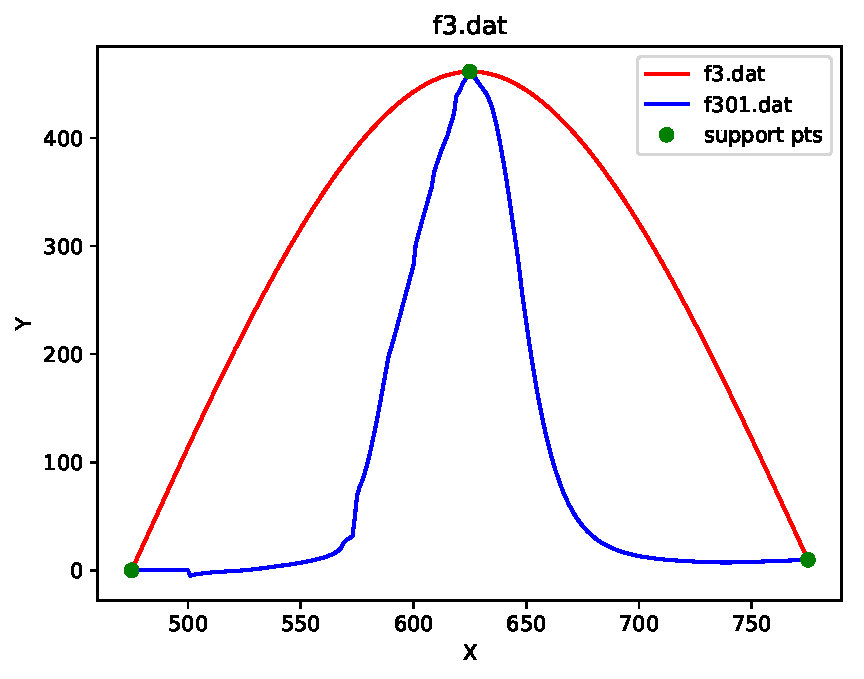
\includegraphics[width=0.55\textwidth]{src/f3.pdf}
    \caption{Result of f3.dat(Spline)}
    \label{fig:f3}
\end{figure}
\begin{figure}[H]
    \centering
    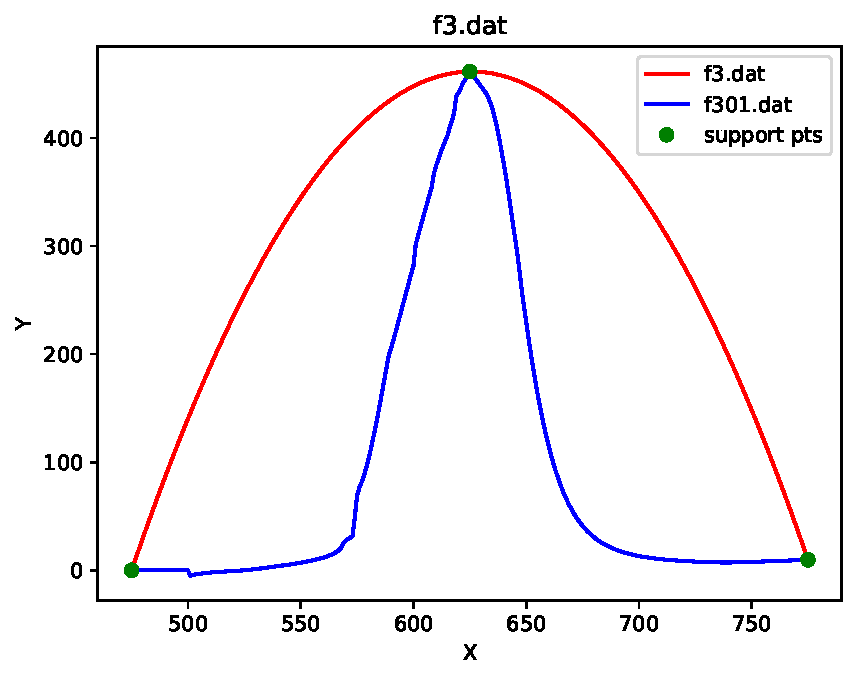
\includegraphics[width=0.55\textwidth]{src/f3_l.pdf}
    \caption{Result of f3.dat(Lagrange)}
    \label{fig:f3l}
\end{figure}
With 3 support points, the result is quite similar. Both of them are second order polynomial. Figure \ref{fig:f5} and \ref{fig:f5l} is the result of
f5.dat.
\begin{figure}[H]
    \centering
    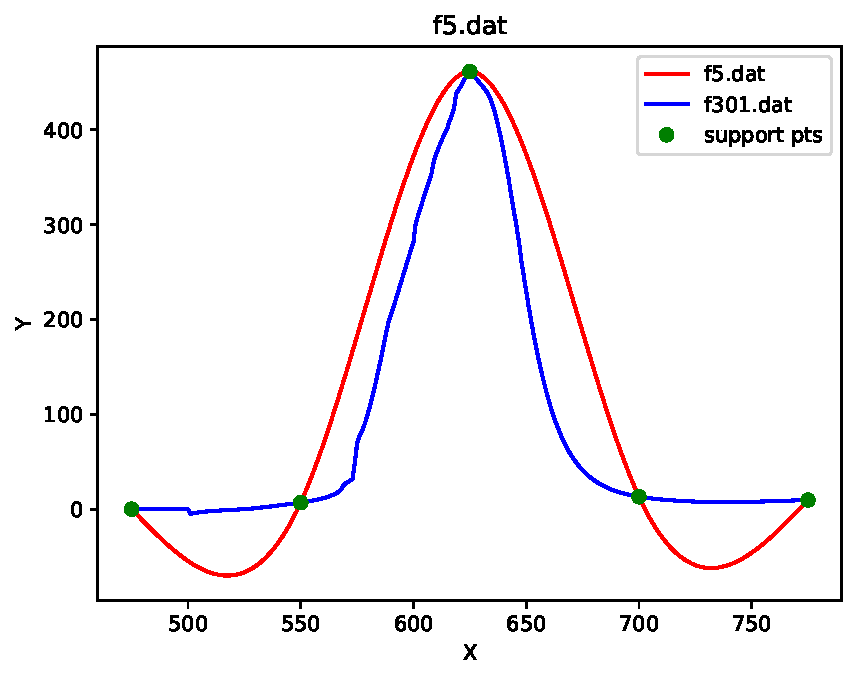
\includegraphics[width=0.55\textwidth]{src/f5.pdf}
    \caption{Result of f5.dat(Spline)}
    \label{fig:f5}
\end{figure}
\begin{figure}[H]
    \centering
    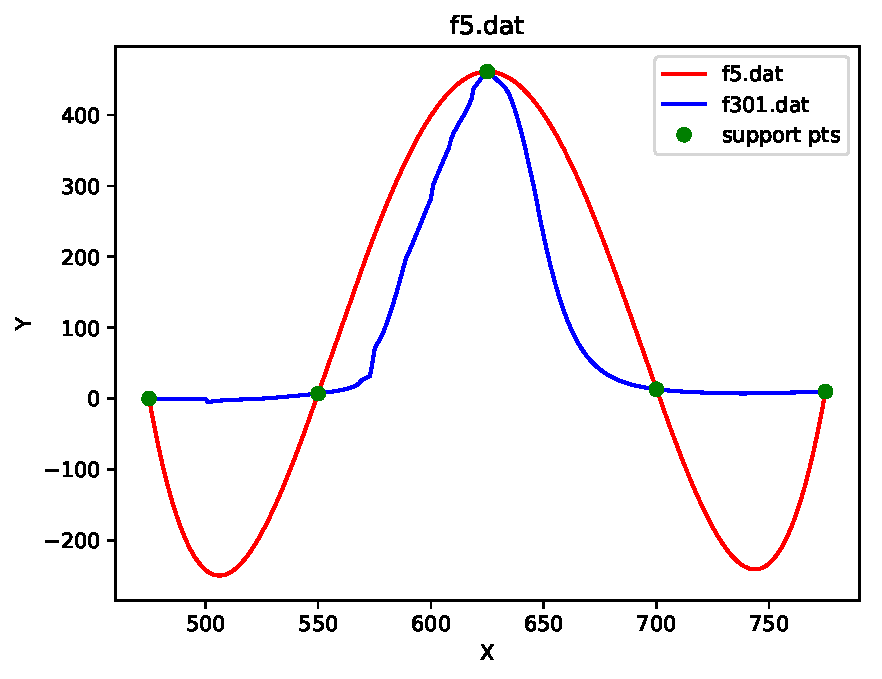
\includegraphics[width=0.55\textwidth]{src/f5_l.pdf}
    \caption{Result of f5.dat(Lagrange)}
    \label{fig:f5l}
\end{figure}
From the two figures, we can find that the oscillation at the two side is more obvious in Langrange and it seems that the result of Spline 
fit the answer better than Lagrange.
\begin{figure}[H]
    \centering
    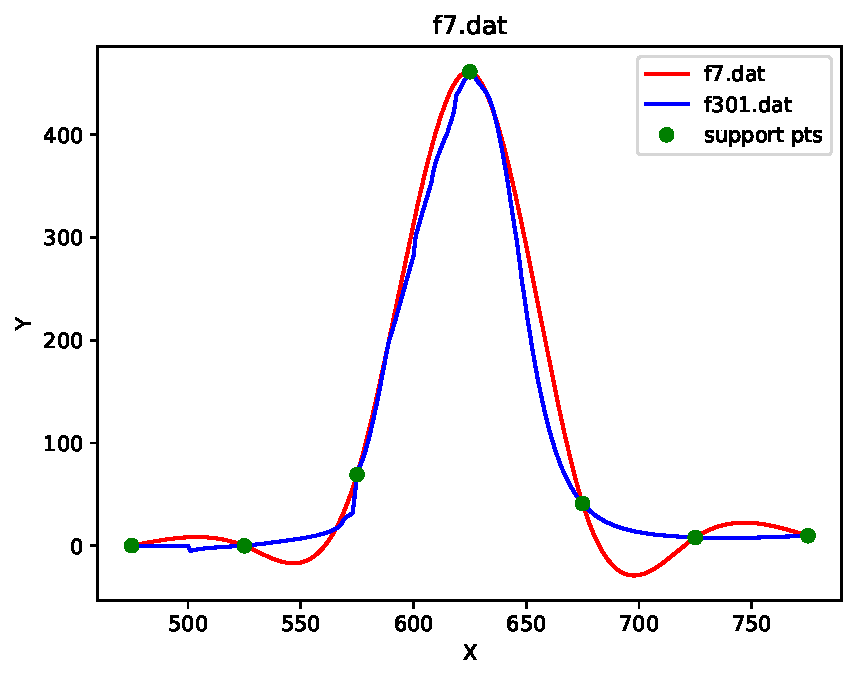
\includegraphics[width=0.55\textwidth]{src/f7.pdf}
    \caption{Result of f7.dat(Spline)}
    \label{fig:f7}
\end{figure}
\begin{figure}[H]
    \centering
    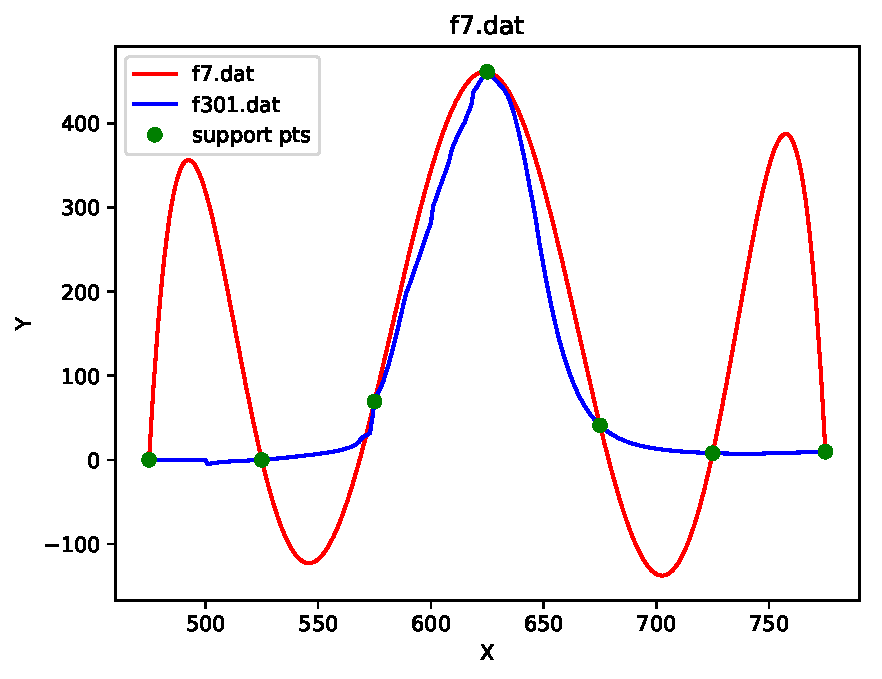
\includegraphics[width=0.55\textwidth]{src/f7_l.pdf}
    \caption{Result of f7.dat(Lagrange)}
    \label{fig:f7l}
\end{figure}
When we see the result from f7.dat(Figure \ref{fig:f7} and \ref{fig:f7l}), the result of Lagrange is a sixth order polunomial, so we can find 6
peak in Figure \ref{fig:f7}. However, the result of Spline is getting more closer to the answer.

\begin{figure}[H]
    \centering
    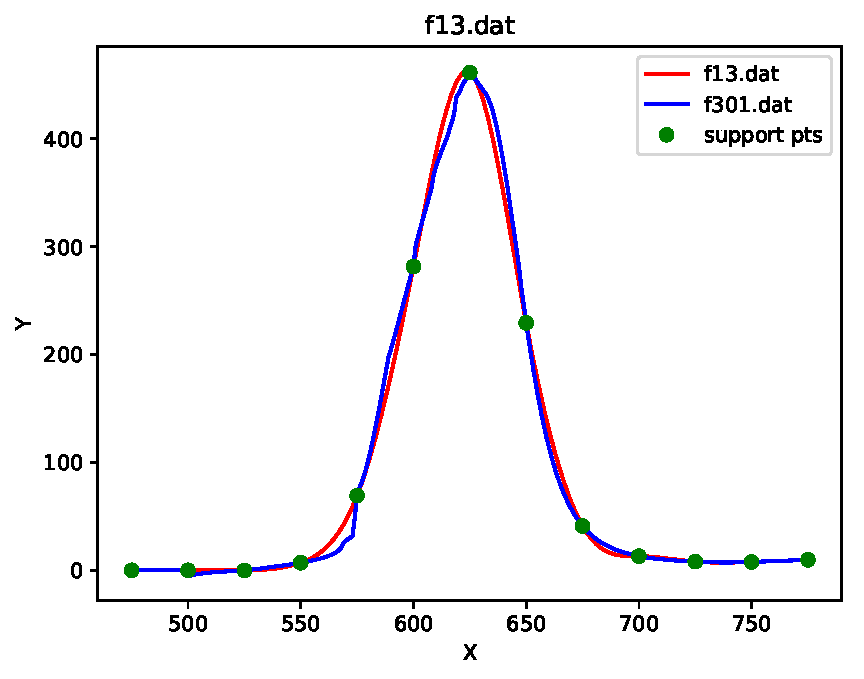
\includegraphics[width=0.55\textwidth]{src/f13.pdf}
    \caption{Result of f13.dat(Spline)}
    \label{fig:f13}
\end{figure}
\begin{figure}[H]
    \centering
    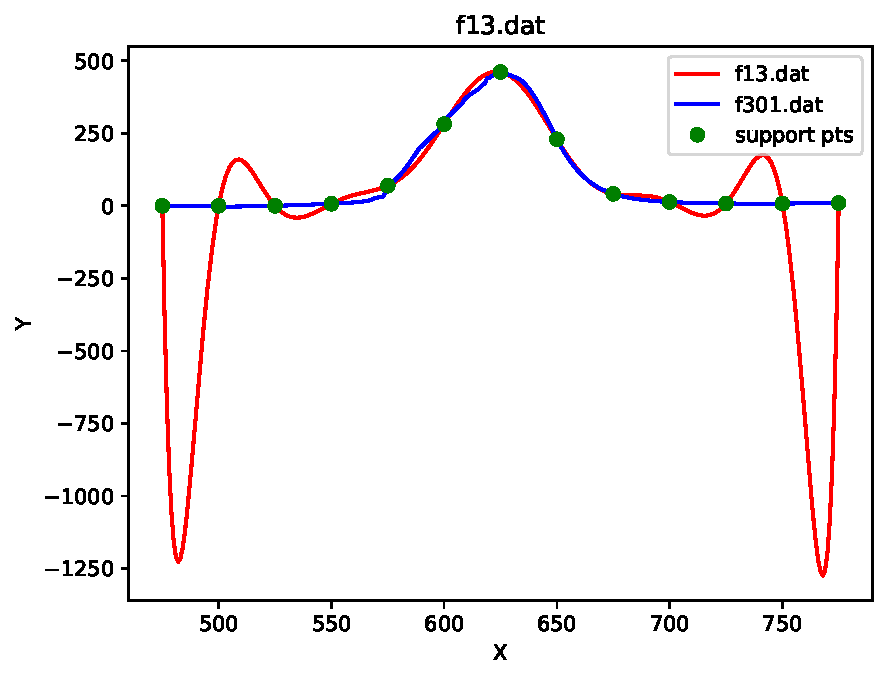
\includegraphics[width=0.55\textwidth]{src/f13_l.pdf}
    \caption{Result of f13.dat(Lagrange)}
    \label{fig:f13l}
\end{figure}
\begin{figure}[H]
    \centering
    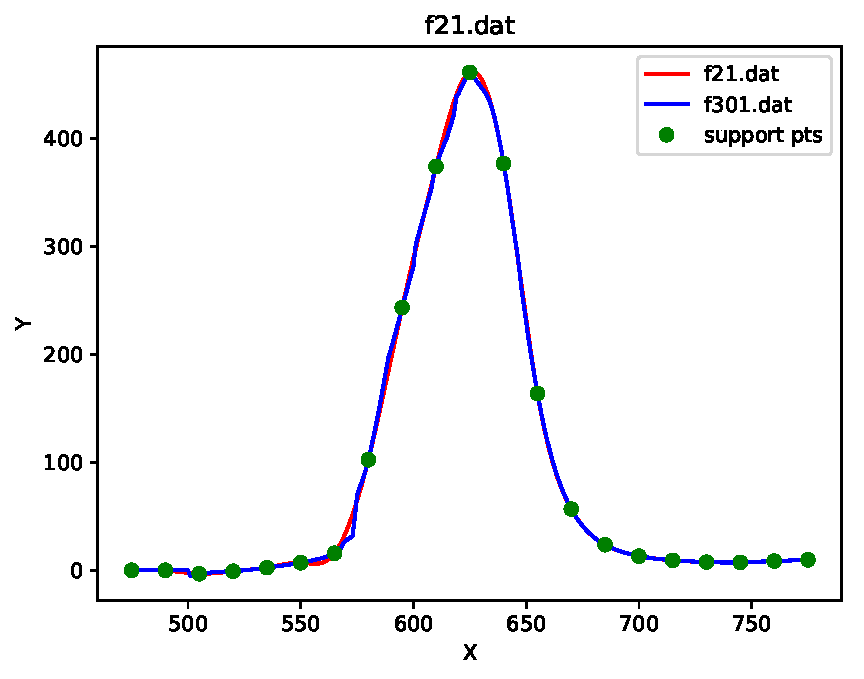
\includegraphics[width=0.55\textwidth]{src/f21.pdf}
    \caption{Result of f21.dat(Spline)}
    \label{fig:f21}
\end{figure}
\begin{figure}[H]
    \centering
    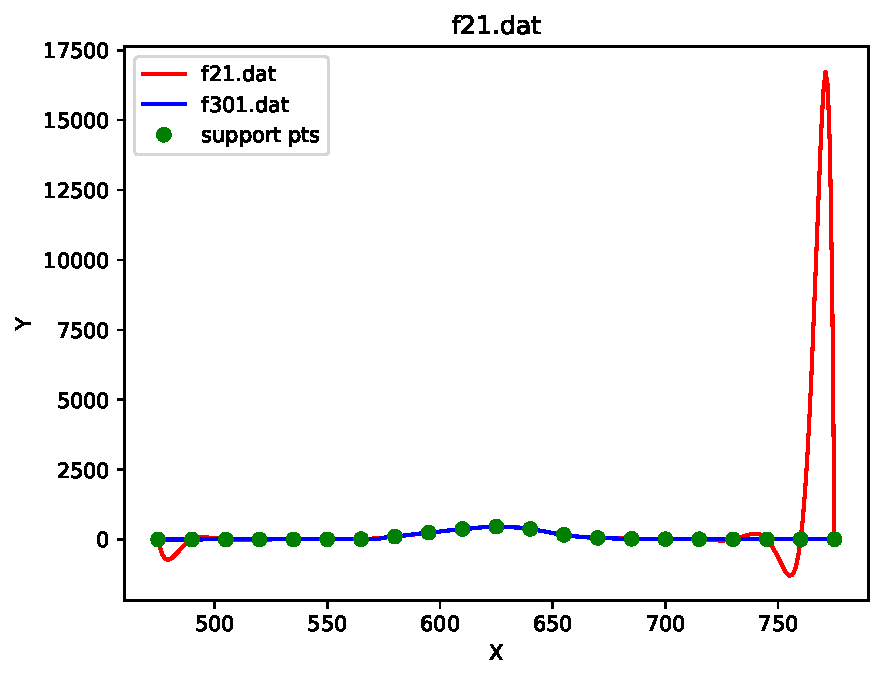
\includegraphics[width=0.55\textwidth]{src/f21_l.pdf}
    \caption{Result of f21.dat(Lagrange)}
    \label{fig:f21l}
\end{figure}
From Figure \ref{fig:f13} and \ref{fig:f21}, Spline fit the answer very well, while Lagrange starts to have huge error at the two side in
Figure \ref{fig:f13l} and \ref{fig:f21l}.

From all figures above, I think Spline Interpolation have better accuracy than Lagrange Interpolation.

\end{document}













